\begin{table}[htbp]
\centering
\caption{Persona Primária}
\label{tab:Table_persona1}
\small
\begin{tabular}{| m{0.2\textwidth} m{0.7\textwidth}|}
\hline \multicolumn{2}{|c|}{\textbf{Identidade}} \\ \hline
& \\

\begin{center} 
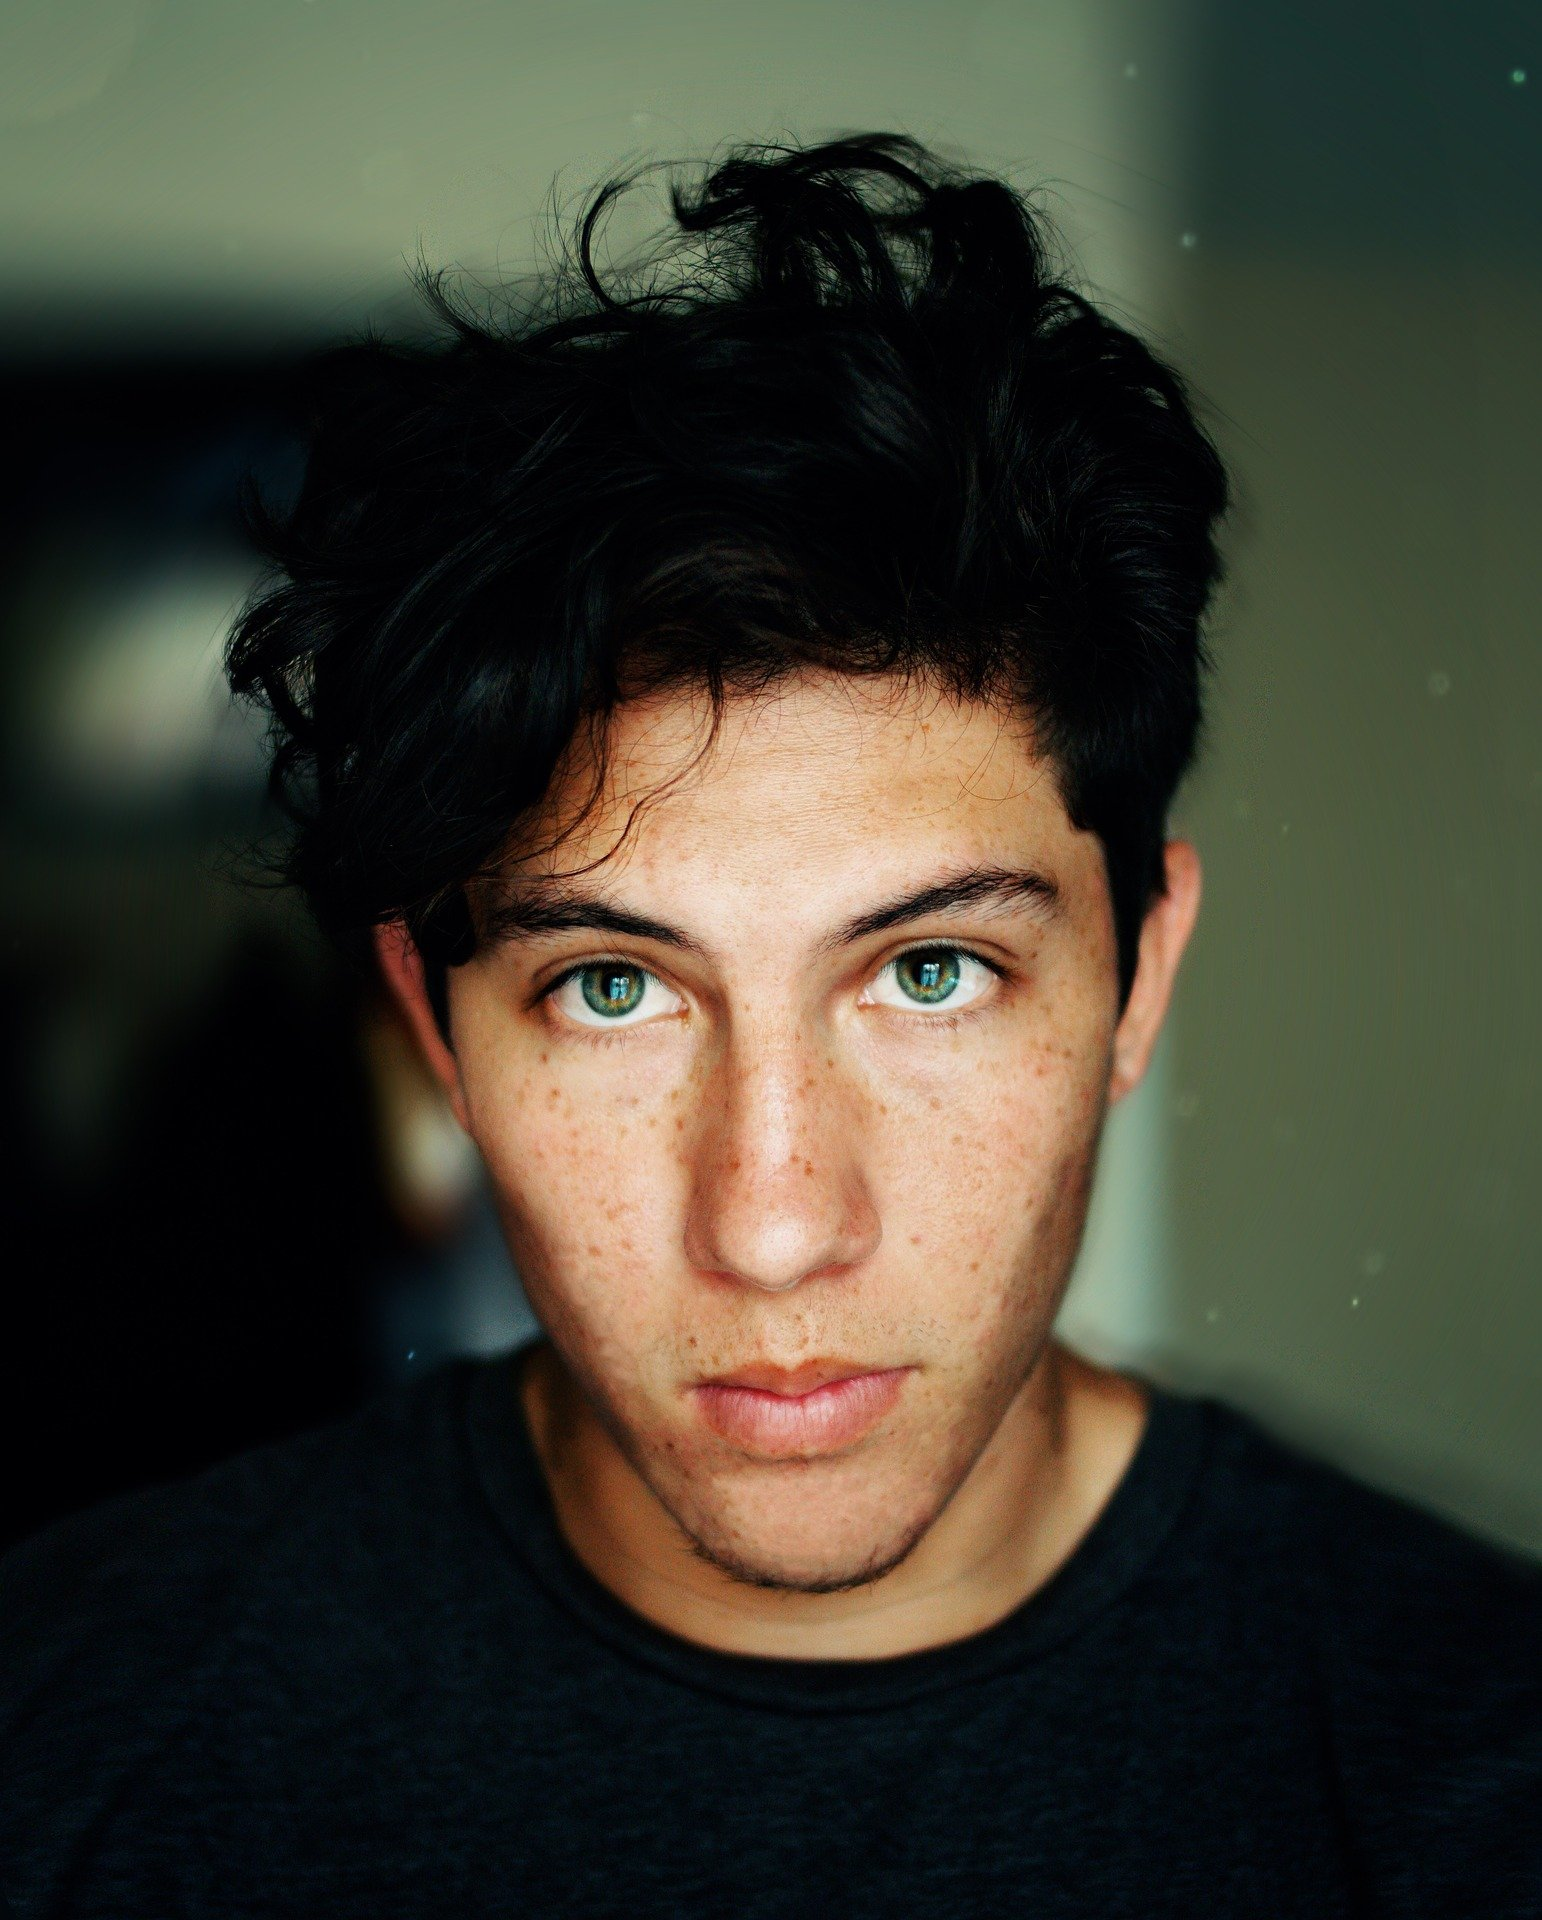
\includegraphics[scale=0.04]{figuras/personas/portrait-3353699_1920.jpg} 
Fonte: Pixabay\tablefootnote{https://pixabay.com/photos/portrait-people-adult-man-face-3353699/}
\end{center} 



&

\textbf{Nome: } Victor Matheus Farias

\textbf{Idade:} 19 anos

\textbf{Ocupação:} Estudante de Engenharia de Software na UnB - Gama.

\\ \hline


\multicolumn{2}{|c|}{\textbf{Descrição}} \\ \hline
\multicolumn{2}{|p{15cm}|}{
    \begin{tabular}[c]{@{}l@{}}\\
    \textbf{Aprender algum conteúdo} é meu o principal objetivo ao usar jogos. Atualmente eu \\\textbf{uso esse tipo de jogo}, mas com uma \textbf{frequência moderada}, não gasto muito tempo\\ com eles. Estou \textbf{começando o curso de IHC} e \textbf{não tenho um conhecimento} \\\textbf{muito técnico} em relação à design de interfaces. O pouco que tenho obtive em \textbf{outras} \\\textbf{disciplinas} da\ faculdade, cursos online e projetos. Quando vou sanar alguma dúvida eu\\ \textbf{pesquiso na internet} e em alguns casos eu pergunto aos \textbf{colegas, o monitor da}\\ \textbf{disciplina ou o professor}.\\
    \\
    Um jogo para aprendizagem, deve me ensinar mesmo que eu erre, \textbf{respondendo às}\\ \textbf{minhas ações}, me ensinando; deve ter um \textbf{design legal}; deve ser \textbf{simples de se}\\ \textbf{aprender a jogar}, \textbf{não tendo regras extensas} e tutorias longos; e \textbf{não deve ser} \\\textbf{muito difícil}. O que mais espero de um jogo assim é sentir \textbf{satisfação} em aprender \\jogando, com uma dose de \textbf{desafios} e \textbf{diversão}. Perceber a \textbf{relevância} do conteúdo \\é algo que me dá \textbf{confiança} que irei atingir meu objetivo de estudo e mesmo não \\gastando muito tempo com jogos, se percebesse bons resultados eu me manteria \textbf{focado}.\\ \\
    \end{tabular}
} \\ \hline
\end{tabular}
\legend{Fonte: Própria Autoria}
\end{table}